\section{Архитектура BBS}

\begin{figure}[h]
    \centering
    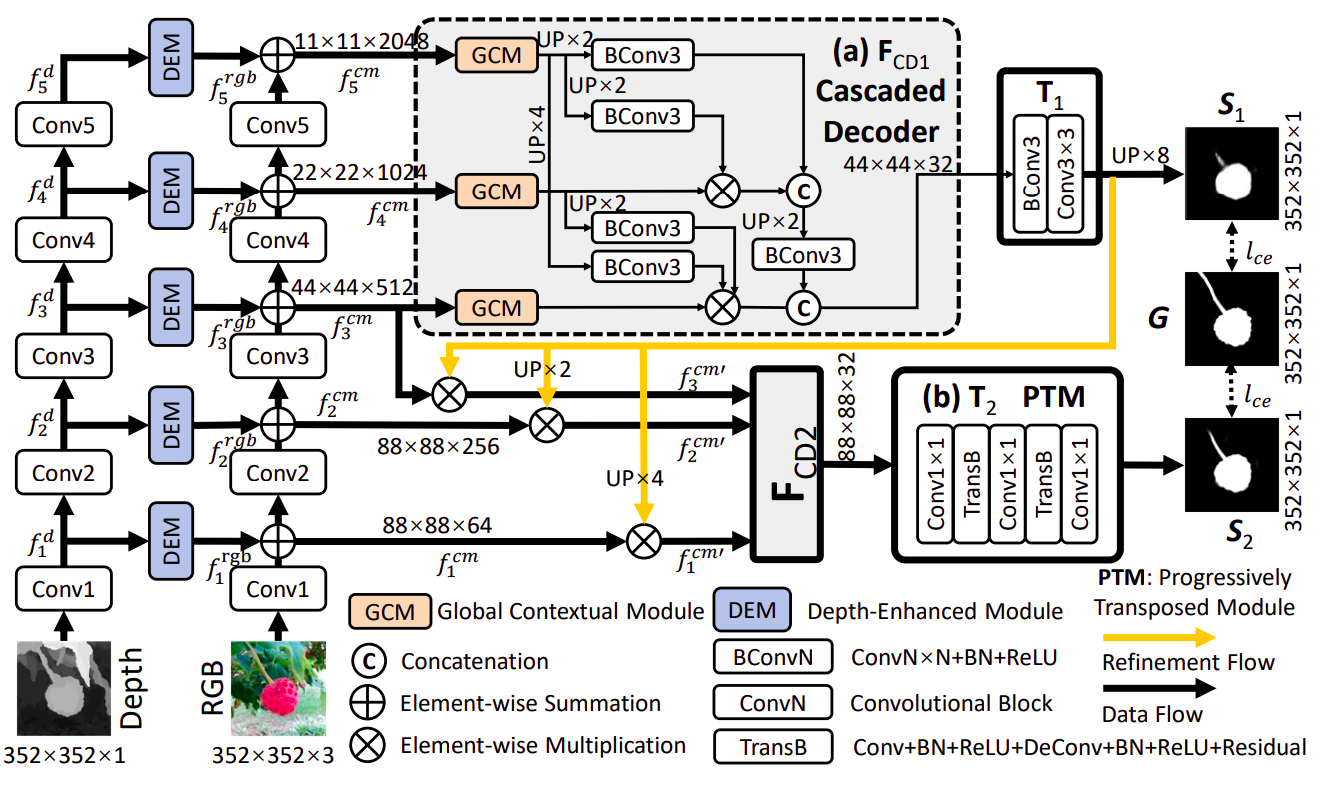
\includegraphics[width=1\textwidth]{bbs}
    \caption{Архитектура сети BBS-Net}
    \label{fig:bbs}
\end{figure}

Летом 2020 года вышла статья \cite{BBS} предлагающая новую архитектуру нейронной сети для решения задачи выявления заметных объектов на изображении 
с использованием карты глубины (RGB-D SOD). Архитектура предполагала использование сразу двух предобученных свёрточных сетей
для выделения признаков (backbones), которые применяются и к RGB, и к карте глубины. Сеть, извлекающая признаки
из карты глубины, "делится" со второй сетью картами признаков, полученных на разных этапах работы через специальный DEM модуль, 
предложенный в статье. Архитектура сети BBS-Net изображена на \ref{fig:bbs}


Свёрточные сети, извлекающие признаки, или экстракторы, разделены на 5 подблоков, эмулируя многоуровневую систему выделения признаков с исходных изображений.
На каждом уровне блок сети, извлекающей признаки из карты глубины, передаёт получившуюся карту признаков $f_i^d, i \in \{1,2,..,5\}$ блоку соседней сети, 
находящемуся на том же уровне, который строит карту $f_i^{rgb}, i \in \{1,2,..,5\}$ . Передача осуществляется через дополнительный модуль DEM, предложенный в работе,
который применяется только к признакам из карты глубины $f_i^d, i \in \{1,2,..,5\}$. 
После этого соответствующие карты признаков поэлементно складываются, образуя кросс-модальные(cross-modality) карты признаков для каждого уровня:

\begin{equation}
    f_i^{cm} = f_i^{rgb} \bigoplus DEM(f_i^{d}), i \in \{1,2,..,5\}
    \label{eq:DEM}
\end{equation}

Таким образом получается, что на каждом уровне признаки, полученные из RGB изображения "обогощаются" признаками из карты глубины.

После этого, карты признаков поступает в два каскадных декодера (cascaded decoder) согласно специальной стратеги. В первый декодер ($F_{CD1}$)
поступают карты признаков с 3,4 и 5-го уровней, а во второй  ($F_{CD2}$) - с 1,2 и 3-го. При этом, до поступления во второй декодер, к каждой карте низкоуровневых 
признаков (1-3 уровня) добавляется ещё и первичная карта заметности (saliency map) $S_1$,которая является результатом работы первого декодера:

\begin{equation}
    S_1 = T_1(F_{CD1}(f_1^{cm},f_2^{cm},f_3^{cm}))
\end{equation}

где $F_{CD1}$ - блок первого декодера, а $T_1$ - простой модуль, содержащий 2 свёрточных слоя, который
нужен для того, чтобы уменьшить число каналов до одного и получить бинарное изображение.

Добавление первичной карты заметности (saliency map) $S_1$ к картам низкоуровневых признаков представляет собой
поэлементное умножение:

\begin{equation}
    f_i^{cm'} = f_i^{cm} \bigotimes S_1, i \in \{1,2,3\}
\end{equation}
Таким образом, мы словно накладываем маску и оставляем из всей карты признаков только ту часть, которая соответствует 
сформированной карте заметности.

Механизм использования первичной карты заметности для уточнения и улучшения финальной карты называется механизмом каскадного уточнения (Cascaded Refinement Mechanism).
Мотивация для его использования лежит в наблюдении за особенностями признаков, получаемых на разных уровнях: высокоуровненвые признаки содержат семантическую информацию,
которая помогает локализовать искомый выделяющийся объект. Тогда как низкоуровневые признаки предоставляют информацию для построения более точных границ на карте значимости.

Далее, карты обновлённые карты признаков $f_i^{cm'}, i \in \{1,2,3\} $ поступает во второй блок декодера $F_{CD2}$, который также оборачивается дополнительными PTM модулем,
состоящим из комбинации свёрток $1 \times 1$, пакетной нормализации (batch norm), функции активации и деконволюции (смотри картинку):

\begin{equation}
    S_2 = T_2(F_{CD2}(f_1^{cm'},f_2^{cm'},f_3^{cm'}))
\end{equation}


Рассмотрим подробнее архитектуру каскадного декодера и модуля DEM

\subsection{Каскадный декодер}
Основная задача декодера - получить искомую карту заметности из карт признаков разного уровня, полученных слиянием признаков,
извлечённых из карты глубины и обработанных DEM модулем, и признаков полученных из RGB изображения.
Каскадный декодер содержит три модуля глобального контекста (Global Context Module, GCM) - по одному на каждую входную карту, после применения которых
используется метод агрегации всех карт признаков в одну. 

Модуль GCM является усовершенствованной версией модуля рецептивного поля(Receptive Fields Block, RFB), предложенного в работе \cite{RFB}
Он состоит из четырёх параллельных веток. Для каждой из них сначала применяется свёртка $1 \time 1$, чтобы уменьшить размер 
канала до 32. После этого для 3 из 4-х веток $k, k \in \{2,3,4\}$ применяется свёртка с размером ядра(kernel size) $2k-1$. За ней 
следует расширенная свёртка(dilated convolutions) $3 \time 3$ с параметром скорости расширения (dilation rate) равным $2k-1$.
Далее, выходы всех чётырёх ветвей конкатенируются вместе, и к ним применяется свёртка $1 \time 1$. 
Результат конкатенируется с исходной картой признаком, полученной из остаточной связи(residual connection) между исходной и финальной картами.
Финальную карту признаков, полученную в результате работы GCM обозначим $f_i^{gcm'}$:

\begin{equation}
    f_i^{gcm} = F_{GCM}(f_i), i \in \{1,2,3\}
\end{equation}

Далее, к полученным картам признаков применяется специальная стратегия группировки и объединения с целью получить единственную
карту заметности. Стратегия включает в себя  поуровневое перемножение и конкатенацию разных признаков, начиная с верхнеуровневых признаков
и заканчивая низкоуровневыми. Стратегия соединения карт признаков представлена на рисунке.

Каждая карта $f_i^{gcm'}$(кроме самой верхнеуровневой) домножается на все верхнеуровневые карты признаков:

\begin{equation}
    f_i^{gcm'} = f_i^{gcm} \bigotimes \prod_{k=i+1}^{k_{max}}Conv(F_{UP}(f_k^{gcm}))
\end{equation}

где $i \in \{1,2,3\}$, $k_{max}=3$ для первого блока декодера с картами признаков $f_i^{cm}, i \in \{1,2,3\}$ , и
$i \in \{3,4,5\}$, $k_{max}=5$ для второго блока с $f_i^{cm}, i \in \{3,4,5\}$. Операция $F_{UP}$ отображает
операцию апсэмплинга (upsampling). Операция $Conv$ - отображает свёртку $3 \time 3$.
На последнем шаге декодера к обновлённым картам признаков $f_i^{gcm'}$  применяется дополнительные операции свёртки и они конкатенируются
в одну карту признаков. 

\begin{equation}
    S = T([f_k^{gcm'}; Conv(F_{UP}[f_{k+1}^{gcm'}; Conv(F_{UP}(f_{k+2}^{gcm'}))])])
\end{equation}

где $S$ - карта заметности, $[x; y]$ - обозначает операцию конкатенации, $k \in \{1,2,3\}$. Операция $T$ - постобработка выхода декодера,
различается для первого и второго декодеров. На первом шаге применяется несколько блоков BConv3 ($T_1$). На втором шаге $T_2$ отображает 
PTM (progressively transposed module) блок для генерации финальной карты заметности.


\subsection{Модуль с расширенной глубиной}

\begin{figure}[h]
    \centering
    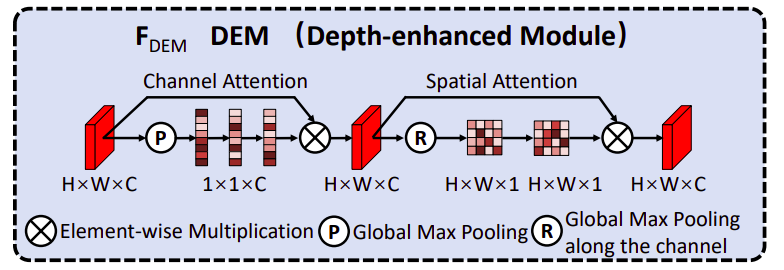
\includegraphics[width=1\textwidth]{dem}
    \caption{Архитектура модуля DEM}
    \label{fig:dem}
\end{figure}

Для эффективного объединения признаков с карты глубины и признаков с RGB изображения нужно решить две проблемы:

\begin{itemize}
    \item проблему совместимости признаков обоих типов 
    \item проблему шума в картах глубины низкого качества 
\end{itemize}

Для решения этих проблем был разработан  модуль увеличения глубины (depth-enhanced module, DEM) на основе
свёрточного модуля с блоком внимания (convolutional block attention module, CBAM), предложенного в работе \cite{Cbam}. 
Архитектура модуля изображена на \ref{fig:dem}.

Модуль DEM применяется к картам признаков $f_i^d$, извлечённых из карты глубины. Карта признаков, полученная в результате его работы
поэлементно складывается с картой признаков $f_i^{rgb}$, как показано в выражении \eqref{eq:DEM}.

Рассмотрим внутреннее устройства DEM модуля. Как изображено на рисунке \ref{fig:dem} модуль состоит из
операции канального внимания(channel attention operation) и операции пространственного внимания(spatial attention operation), идущих последовательно:

\begin{equation}
    F_{DEM}(f_i^d)=S_{att}(C_{att}(f_i^d))
\end{equation}

где $C_{att}$ и $S_{att}$ обозначает операцию и канального внимания операцию пространственного внимания
соответственно.

Операция канального внимания реализована следующим образом:

\begin{equation}
    C_{att}(f)=M(P_{max}(f)) \bigotimes f
\end{equation}

где $P_{max}$ обозначает операцию глобального пулинга для каждого "слоя"
карты признаков, $M$ обозначает двухслойный перцептрон, 
результат которого перемножается с изначальной картой признаков $f$.

Операция пространственного внимания реализована как 

\begin{equation}
    S_{att}(f)=Conv(R_{max}(f)) \bigotimes f
\end{equation}

где $R_{max}$ обозначает операцию глобального пулинга, применённого к 
каждому каналу.

В следующей части работы мы рассмотрим возможные улучшения архитектуры и тренировочного процесса модели BBS-Net.